% End-to-end identity-establishment latency -- sub-sub-section.
% Drop into your manuscript with: % End-to-end identity-establishment latency -- sub-sub-section.
% Drop into your manuscript with: % End-to-end identity-establishment latency -- sub-sub-section.
% Drop into your manuscript with: % End-to-end identity-establishment latency -- sub-sub-section.
% Drop into your manuscript with: \input{path/to/identity_establishment_latency.tex}
% Requires: \usepackage{booktabs} and \graphicspath including the figures/ folder.
\subsubsection{End-to-End Identity-Establishment Latency}
\label{sec:eval-establishment}

We compare the end-to-end first-time identity-establishment latency of four
architectures on AWS EC2 \texttt{us-east-1} against Sui Devnet, with submission
semantics fixed to \texttt{WaitForEffectsCert} for fairness across all on-chain
baselines. To enable apples-to-apples comparison, all four baselines are
measured as Node.js processes; for zkEHR this means a measurement harness that
imports the same multi-authority salt fan-out, the same Mysten Devnet prover
endpoint, and the same Move package the production system uses, but replaces
the React/Vite UI shell with direct Node orchestration. Table~\ref{tab:identity-establishment}
reports the aggregate distribution and Figure~\ref{fig:cmp-phases} attributes
the mean to five protocol phases.

\begin{table}[htbp]
\centering
\caption{End-to-end identity-establishment latency (ms).}
\label{tab:identity-establishment}
\small
\setlength{\tabcolsep}{4pt}
\begin{tabular}{l@{\hspace{6pt}}r r r r r r}
\toprule
\textbf{Baseline} & $n$ & \textbf{mean} & \textbf{std} & \textbf{p50} & \textbf{p95} & \textbf{p99} \\
\midrule
OIDC-only & 100 & 240 & 16.9 & 237.2 & 268.4 & 284.1 \\
Private-key DID/VC & 100 & 319 & 72.3 & 313.3 & 392.5 & 468.5 \\
zkLogin-only & 100 & 3416 & 295.4 & 3507.1 & 3826.3 & 3926.9 \\
zkEHR (proposed) & 100 & 3381 & 284.5 & 3453.9 & 3779.5 & 3859.7 \\
\bottomrule
\end{tabular}
\end{table}

\begin{figure}[htbp]
\centering
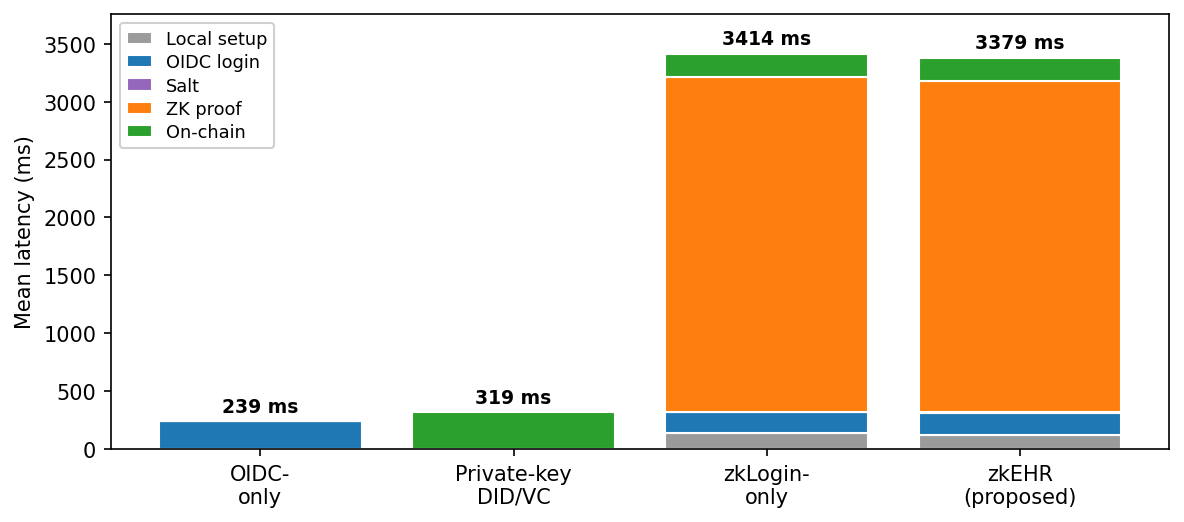
\includegraphics[width=0.95\linewidth]{figures/comparison_phases.png}
\caption{Per-phase contribution to identity-establishment latency. The Mysten
Labs ZK prover dominates both zk-anchored systems; zkEHR's overhead beyond
zkLogin-only is the multi-authority salt fan-out plus orchestration.}
\label{fig:cmp-phases}
\end{figure}

The four protocols trace a clean cost--property ladder. OIDC-only
(240\,ms) trusts a single OpenID Provider; private-key DID/VC
(319\,ms) adds blockchain auditability through a Sui transaction;
zkLogin-only (3416\,ms) further unlinks identity from key custody,
paying the Mysten Devnet Groth16 proof cost (84.5\% of total)
that binds the JWT to a Sui address. zkEHR (3381\,ms) layers
multi-authority salt across $N\!=\!4$ institutions on top of zkLogin; the
salt fan-out contributes 5.5\,ms (versus 0.07\,ms for
single-authority salt). The zkEHR mean is statistically indistinguishable
from zkLogin-only: the inter-baseline difference ($\sim\!35$\,ms) is
roughly $1/8$ of either baseline's standard deviation
(295.4\,ms and 284.5\,ms respectively), which is dominated by
Mysten prover RTT variance shared by both systems. zkEHR therefore obtains
the resilience property of multi-authority salt at no measurable wall-clock
cost over the single-authority zkLogin baseline, while remaining
$14.1\times$ slower than OIDC-only as the unavoidable price of
zk-anchored decentralized identity.

% Requires: \usepackage{booktabs} and \graphicspath including the figures/ folder.
\subsubsection{End-to-End Identity-Establishment Latency}
\label{sec:eval-establishment}

We compare the end-to-end first-time identity-establishment latency of four
architectures on AWS EC2 \texttt{us-east-1} against Sui Devnet, with submission
semantics fixed to \texttt{WaitForEffectsCert} for fairness across all on-chain
baselines. To enable apples-to-apples comparison, all four baselines are
measured as Node.js processes; for zkEHR this means a measurement harness that
imports the same multi-authority salt fan-out, the same Mysten Devnet prover
endpoint, and the same Move package the production system uses, but replaces
the React/Vite UI shell with direct Node orchestration. Table~\ref{tab:identity-establishment}
reports the aggregate distribution and Figure~\ref{fig:cmp-phases} attributes
the mean to five protocol phases.

\begin{table}[htbp]
\centering
\caption{End-to-end identity-establishment latency (ms).}
\label{tab:identity-establishment}
\small
\setlength{\tabcolsep}{4pt}
\begin{tabular}{l@{\hspace{6pt}}r r r r r r}
\toprule
\textbf{Baseline} & $n$ & \textbf{mean} & \textbf{std} & \textbf{p50} & \textbf{p95} & \textbf{p99} \\
\midrule
OIDC-only & 100 & 240 & 16.9 & 237.2 & 268.4 & 284.1 \\
Private-key DID/VC & 100 & 319 & 72.3 & 313.3 & 392.5 & 468.5 \\
zkLogin-only & 100 & 3416 & 295.4 & 3507.1 & 3826.3 & 3926.9 \\
zkEHR (proposed) & 100 & 3381 & 284.5 & 3453.9 & 3779.5 & 3859.7 \\
\bottomrule
\end{tabular}
\end{table}

\begin{figure}[htbp]
\centering
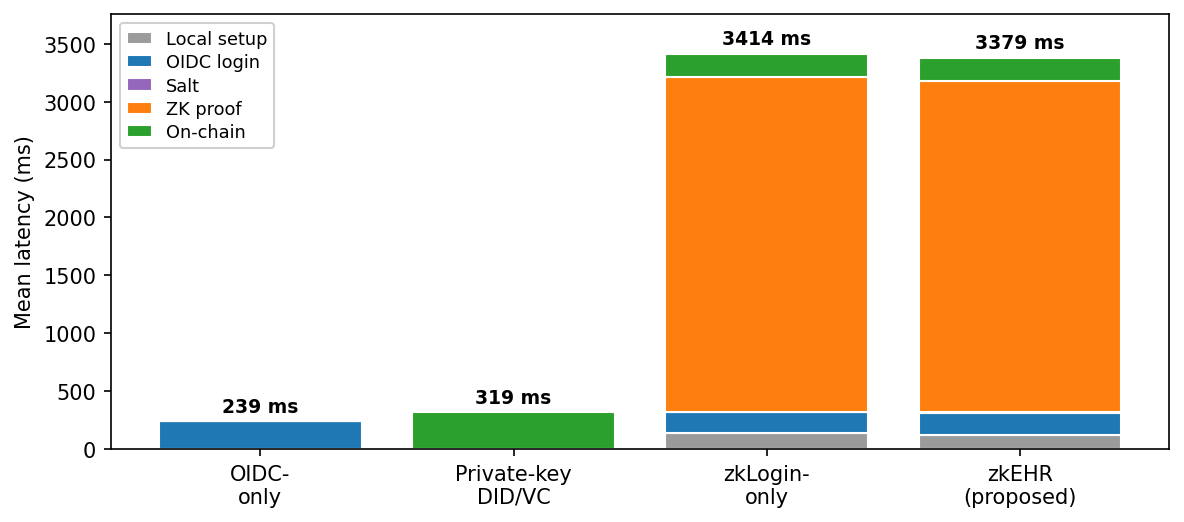
\includegraphics[width=0.95\linewidth]{figures/comparison_phases.png}
\caption{Per-phase contribution to identity-establishment latency. The Mysten
Labs ZK prover dominates both zk-anchored systems; zkEHR's overhead beyond
zkLogin-only is the multi-authority salt fan-out plus orchestration.}
\label{fig:cmp-phases}
\end{figure}

The four protocols trace a clean cost--property ladder. OIDC-only
(240\,ms) trusts a single OpenID Provider; private-key DID/VC
(319\,ms) adds blockchain auditability through a Sui transaction;
zkLogin-only (3416\,ms) further unlinks identity from key custody,
paying the Mysten Devnet Groth16 proof cost (84.5\% of total)
that binds the JWT to a Sui address. zkEHR (3381\,ms) layers
multi-authority salt across $N\!=\!4$ institutions on top of zkLogin; the
salt fan-out contributes 5.5\,ms (versus 0.07\,ms for
single-authority salt). The zkEHR mean is statistically indistinguishable
from zkLogin-only: the inter-baseline difference ($\sim\!35$\,ms) is
roughly $1/8$ of either baseline's standard deviation
(295.4\,ms and 284.5\,ms respectively), which is dominated by
Mysten prover RTT variance shared by both systems. zkEHR therefore obtains
the resilience property of multi-authority salt at no measurable wall-clock
cost over the single-authority zkLogin baseline, while remaining
$14.1\times$ slower than OIDC-only as the unavoidable price of
zk-anchored decentralized identity.

% Requires: \usepackage{booktabs} and \graphicspath including the figures/ folder.
\subsubsection{End-to-End Identity-Establishment Latency}
\label{sec:eval-establishment}

We compare the end-to-end first-time identity-establishment latency of four
architectures on AWS EC2 \texttt{us-east-1} against Sui Devnet, with submission
semantics fixed to \texttt{WaitForEffectsCert} for fairness across all on-chain
baselines. To enable apples-to-apples comparison, all four baselines are
measured as Node.js processes; for zkEHR this means a measurement harness that
imports the same multi-authority salt fan-out, the same Mysten Devnet prover
endpoint, and the same Move package the production system uses, but replaces
the React/Vite UI shell with direct Node orchestration. Table~\ref{tab:identity-establishment}
reports the aggregate distribution and Figure~\ref{fig:cmp-phases} attributes
the mean to five protocol phases.

\begin{table}[htbp]
\centering
\caption{End-to-end identity-establishment latency (ms).}
\label{tab:identity-establishment}
\small
\setlength{\tabcolsep}{4pt}
\begin{tabular}{l@{\hspace{6pt}}r r r r r r}
\toprule
\textbf{Baseline} & $n$ & \textbf{mean} & \textbf{std} & \textbf{p50} & \textbf{p95} & \textbf{p99} \\
\midrule
OIDC-only & 100 & 240 & 16.9 & 237.2 & 268.4 & 284.1 \\
Private-key DID/VC & 100 & 319 & 72.3 & 313.3 & 392.5 & 468.5 \\
zkLogin-only & 100 & 3416 & 295.4 & 3507.1 & 3826.3 & 3926.9 \\
zkEHR (proposed) & 100 & 3381 & 284.5 & 3453.9 & 3779.5 & 3859.7 \\
\bottomrule
\end{tabular}
\end{table}

\begin{figure}[htbp]
\centering
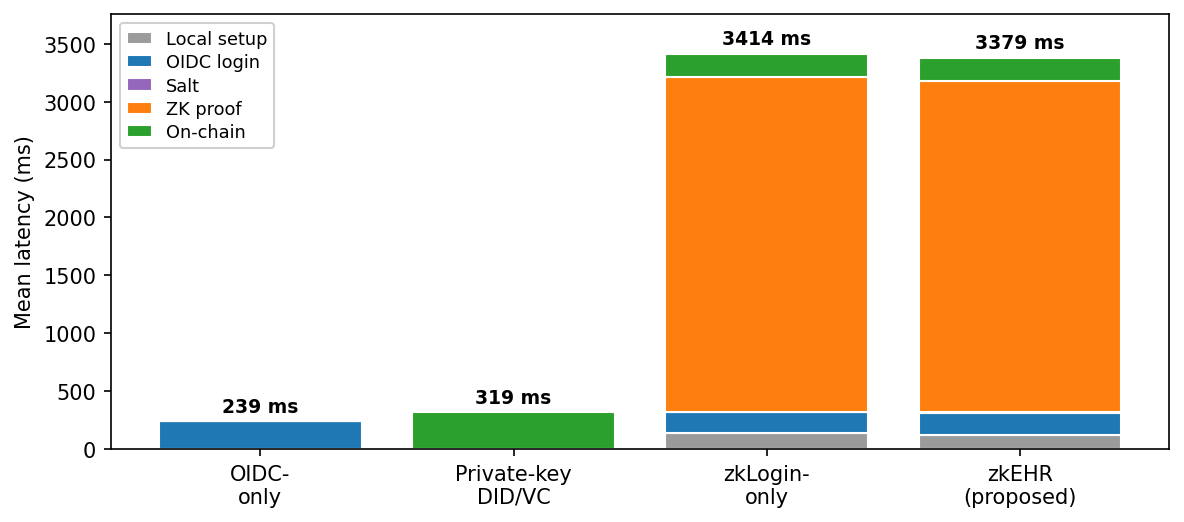
\includegraphics[width=0.95\linewidth]{figures/comparison_phases.png}
\caption{Per-phase contribution to identity-establishment latency. The Mysten
Labs ZK prover dominates both zk-anchored systems; zkEHR's overhead beyond
zkLogin-only is the multi-authority salt fan-out plus orchestration.}
\label{fig:cmp-phases}
\end{figure}

The four protocols trace a clean cost--property ladder. OIDC-only
(240\,ms) trusts a single OpenID Provider; private-key DID/VC
(319\,ms) adds blockchain auditability through a Sui transaction;
zkLogin-only (3416\,ms) further unlinks identity from key custody,
paying the Mysten Devnet Groth16 proof cost (84.5\% of total)
that binds the JWT to a Sui address. zkEHR (3381\,ms) layers
multi-authority salt across $N\!=\!4$ institutions on top of zkLogin; the
salt fan-out contributes 5.5\,ms (versus 0.07\,ms for
single-authority salt). The zkEHR mean is statistically indistinguishable
from zkLogin-only: the inter-baseline difference ($\sim\!35$\,ms) is
roughly $1/8$ of either baseline's standard deviation
(295.4\,ms and 284.5\,ms respectively), which is dominated by
Mysten prover RTT variance shared by both systems. zkEHR therefore obtains
the resilience property of multi-authority salt at no measurable wall-clock
cost over the single-authority zkLogin baseline, while remaining
$14.1\times$ slower than OIDC-only as the unavoidable price of
zk-anchored decentralized identity.

% Requires: \usepackage{booktabs} and \graphicspath including the figures/ folder.
\subsubsection{End-to-End Identity-Establishment Latency}
\label{sec:eval-establishment}

We compare the end-to-end first-time identity-establishment latency of four
architectures on AWS EC2 \texttt{us-east-1} against Sui Devnet, with submission
semantics fixed to \texttt{WaitForEffectsCert} for fairness across all on-chain
baselines. To enable apples-to-apples comparison, all four baselines are
measured as Node.js processes; for zkEHR this means a measurement harness that
imports the same multi-authority salt fan-out, the same Mysten Devnet prover
endpoint, and the same Move package the production system uses, but replaces
the React/Vite UI shell with direct Node orchestration. Table~\ref{tab:identity-establishment}
reports the aggregate distribution and Figure~\ref{fig:cmp-phases} attributes
the mean to five protocol phases.

\begin{table}[htbp]
\centering
\caption{End-to-end identity-establishment latency (ms).}
\label{tab:identity-establishment}
\small
\setlength{\tabcolsep}{4pt}
\begin{tabular}{l@{\hspace{6pt}}r r r r r r}
\toprule
\textbf{Baseline} & $n$ & \textbf{mean} & \textbf{std} & \textbf{p50} & \textbf{p95} & \textbf{p99} \\
\midrule
OIDC-only & 100 & 240 & 16.9 & 237.2 & 268.4 & 284.1 \\
Private-key DID/VC & 100 & 319 & 72.3 & 313.3 & 392.5 & 468.5 \\
zkLogin-only & 100 & 3416 & 295.4 & 3507.1 & 3826.3 & 3926.9 \\
zkEHR (proposed) & 100 & 3381 & 284.5 & 3453.9 & 3779.5 & 3859.7 \\
\bottomrule
\end{tabular}
\end{table}

\begin{figure}[htbp]
\centering
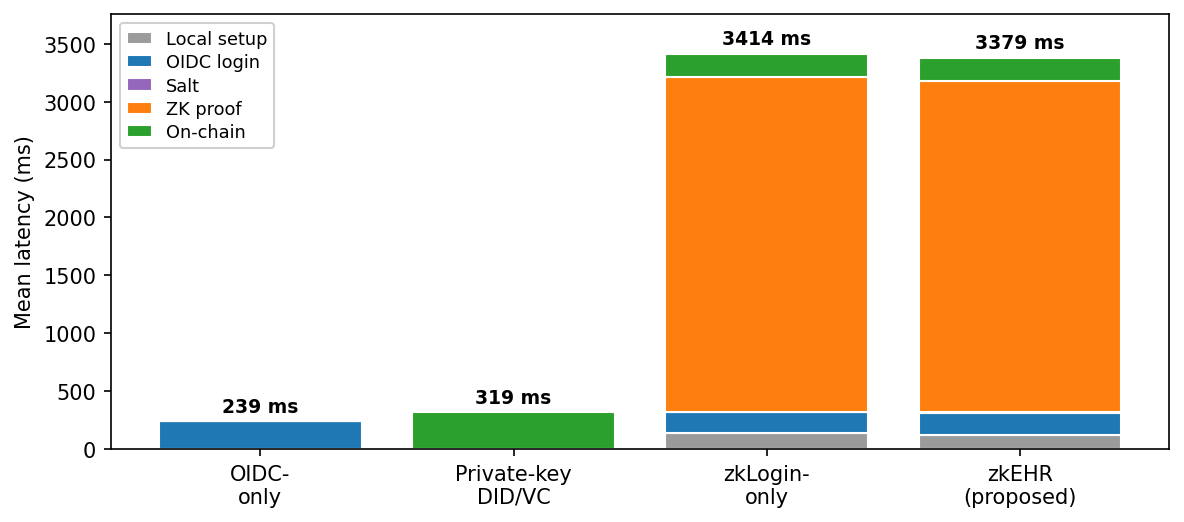
\includegraphics[width=0.95\linewidth]{figures/comparison_phases.png}
\caption{Per-phase contribution to identity-establishment latency. The Mysten
Labs ZK prover dominates both zk-anchored systems; zkEHR's overhead beyond
zkLogin-only is the multi-authority salt fan-out plus orchestration.}
\label{fig:cmp-phases}
\end{figure}

The four protocols trace a clean cost--property ladder. OIDC-only
(240\,ms) trusts a single OpenID Provider; private-key DID/VC
(319\,ms) adds blockchain auditability through a Sui transaction;
zkLogin-only (3416\,ms) further unlinks identity from key custody,
paying the Mysten Devnet Groth16 proof cost (84.5\% of total)
that binds the JWT to a Sui address. zkEHR (3381\,ms) layers
multi-authority salt across $N\!=\!4$ institutions on top of zkLogin; the
salt fan-out contributes 5.5\,ms (versus 0.07\,ms for
single-authority salt). The zkEHR mean is statistically indistinguishable
from zkLogin-only: the inter-baseline difference ($\sim\!35$\,ms) is
roughly $1/8$ of either baseline's standard deviation
(295.4\,ms and 284.5\,ms respectively), which is dominated by
Mysten prover RTT variance shared by both systems. zkEHR therefore obtains
the resilience property of multi-authority salt at no measurable wall-clock
cost over the single-authority zkLogin baseline, while remaining
$14.1\times$ slower than OIDC-only as the unavoidable price of
zk-anchored decentralized identity.
